\documentclass{llncs}


 %%%% Compression Light+: LNCS margin reduced by +/-7mm along all edges (RG).
%\textwidth=130mm   % LNCS: 122mm
%\textheight=203mm  % LNCS: 193mm

\renewcommand{\baselinestretch}{0.97}

\usepackage{amssymb}
\usepackage{amsmath}
\usepackage[sans]{dsfont}
\usepackage{color}
\usepackage{ifthen}
\usepackage{xspace}
\usepackage{listings}
\usepackage{fancyvrb}
\usepackage{multirow}
\usepackage[pdftex]{graphicx}

%\input{macros}

\pagestyle{plain}

%\lstset{mathescape=true,language=Java,basicstyle=\tt,keywordstyle=\bf}
\lstset{language=Python,
        basicstyle=\scriptsize\ttfamily,
        keywordstyle=\color{blue}, % I couldn't find a way to make chars both bold and tt
        frame=none,
        stringstyle=\color{blue},
        fancyvrb=true,
        xleftmargin=20pt,xrightmargin=20pt,
        showstringspaces=false}

\setlength{\tabcolsep}{1ex}


%\renewcommand{\baselinestretch}{.98}
\newboolean{showcomments}
\setboolean{showcomments}{false}
\ifthenelse{\boolean{showcomments}}
  {\newcommand{\nb}[2]{
    \fbox{\bfseries\sffamily\scriptsize#1}
    {\sf\small$\blacktriangleright$\textit{#2}$\blacktriangleleft$}
   }
   \newcommand{\version}{\emph{\scriptsize$-$Id: main.tex 19055 2008-06-05 11:20:31Z cfbolz $-$}}
  }
  {\newcommand{\nb}[2]{}
   \newcommand{\version}{}
  }

\newcommand\dacom[1]{\nb{DA}{#1}}
\newcommand\cfbolz[1]{\nb{CFB}{#1}}
\newcommand\anto[1]{\nb{ANTO}{#1}}
\newcommand\arigo[1]{\nb{AR}{#1}}
\newcommand{\commentout}[1]{}

\let\oldcite=\cite

\renewcommand\cite[1]{\ifthenelse{\equal{#1}{XXX}}{[citation~needed]}{\oldcite{#1}}}


\begin{document}
\title{Automatic generation of JIT compilers for dynamic languages
  in .NET\thanks{This work has been partially
supported by MIUR EOS DUE - Extensible Object Systems for Dynamic and
Unpredictable Environments and by the EU-funded project: IST 004779 PyPy
(PyPy: Implementing Python in Python).}}


\author{Davide Ancona\inst{1} \and Carl Friedrich Bolz\inst{2} \and Antonio Cuni\inst{1} \and Armin Rigo\inst{2}}

\institute{DISI, University of Genova, Italy 
\and 
Softwaretechnik und Programmiersprachen
 Heinrich-Heine-Universit\"at D\"usseldorf}

\maketitle

\commentout{
\section{Tentative structure}
\begin{itemize}
  \item Introduction \& background; main contributions:
    \begin{itemize}
      \item Promotion
      \item (unboxing)
      \item JIT layering
    \end{itemize}
  \item How the generated JITs work
    \begin{itemize}
      \item Promotion: allows intermixing compile-time and runtime; how to
        compare with polymorphic inline caches and partial evaluation
      \item unboxing: how they compare with tracing JITs
      \item (don't talk about merging)
    \end{itemize}
  \item .NET backend
  \item How the JIT generator works
  \item Benchmarks (TLC)
  \item Future works
  \item Conclusions
\end{itemize}
}    

\begin{abstract}
Writing an optimizing static compiler for dynamic languages is not an
easy task, since quite complex static analysis is required.
On the other hand, recent developments show that JIT compilers 
can exploit runtime type information to generate quite efficient code.
Unfortunately, writing a JIT compiler is far from being simple.
 
In this paper we report our positive experience with automatic generation
of JIT compilers as supported by the PyPy infrastructure, by
focusing  on JIT compilation for .NET.
The paper presents two main and novel contributions: we show that
partial evaluation can be used in practice for generating a JIT compiler,
and we experiment with the potentiality offered by the ability to
add a further level of JIT compilation on top of .NET.

The practicality of the approach is demonstrated by showing some
promising experiments done with benchmarks written in a simple dynamic language.
\end{abstract}

% LocalWords:  JIT PyPy

\section{Introduction}
The easiest way to implement a dynamic language such as Python is to write an
interpreter; however, interpreters are slow.

The alternative is to write a compiler; writing a compiler that targets a high
level virtual machine like CLI or JVM is easier than targeting a real CPU, but
it still requires a lot of work, as IronPython, Jython, JRuby demonstrate.

Moreover, writing a static compiler is often not enough to get high
performance; IronPython and JRuby are going in the direction of JIT compiling
specialized versions of the code depending on the actual values/types seen at
runtime; this approach seems to work, but writing it manually requires an
enormous effort.

PyPy's approach \cite{RiBo07_223} is to automatize the generation of JIT compilers in order
to minimize the effort required to get a fast implementation of a
dynamic language; automatic generation of JIT compilers is done with
the help of partial evaluation techniques and requires the user only
to provide an interpreter with some manual annotations which hint
the generator how interpretation and JIT compilation has to be interleaved. 

More precisely, in this paper we focus on the ability of generating a JIT compiler able to emit code
for the .NET virtual machine. To our knowledge, this is the first experiment with an interpreter with
two \emph{layers} of JIT compilation, since, before being executed, the
emitted code is eventually compiled again by .NET's own JIT compiler.

The contributions of this paper are twofold: (1) \emph{promotion} is a
generalization of polymorphic inline caches that make partial evaluation
practical for dynamic languages; (2) we demonstrated that the idea of
\emph{JIT layering} can give good results, as dynamic languages can be even
faster than their static counterparts.

\subsection{PyPy and RPython}

\commentout{
\begin{figure}[h]
\begin{center}
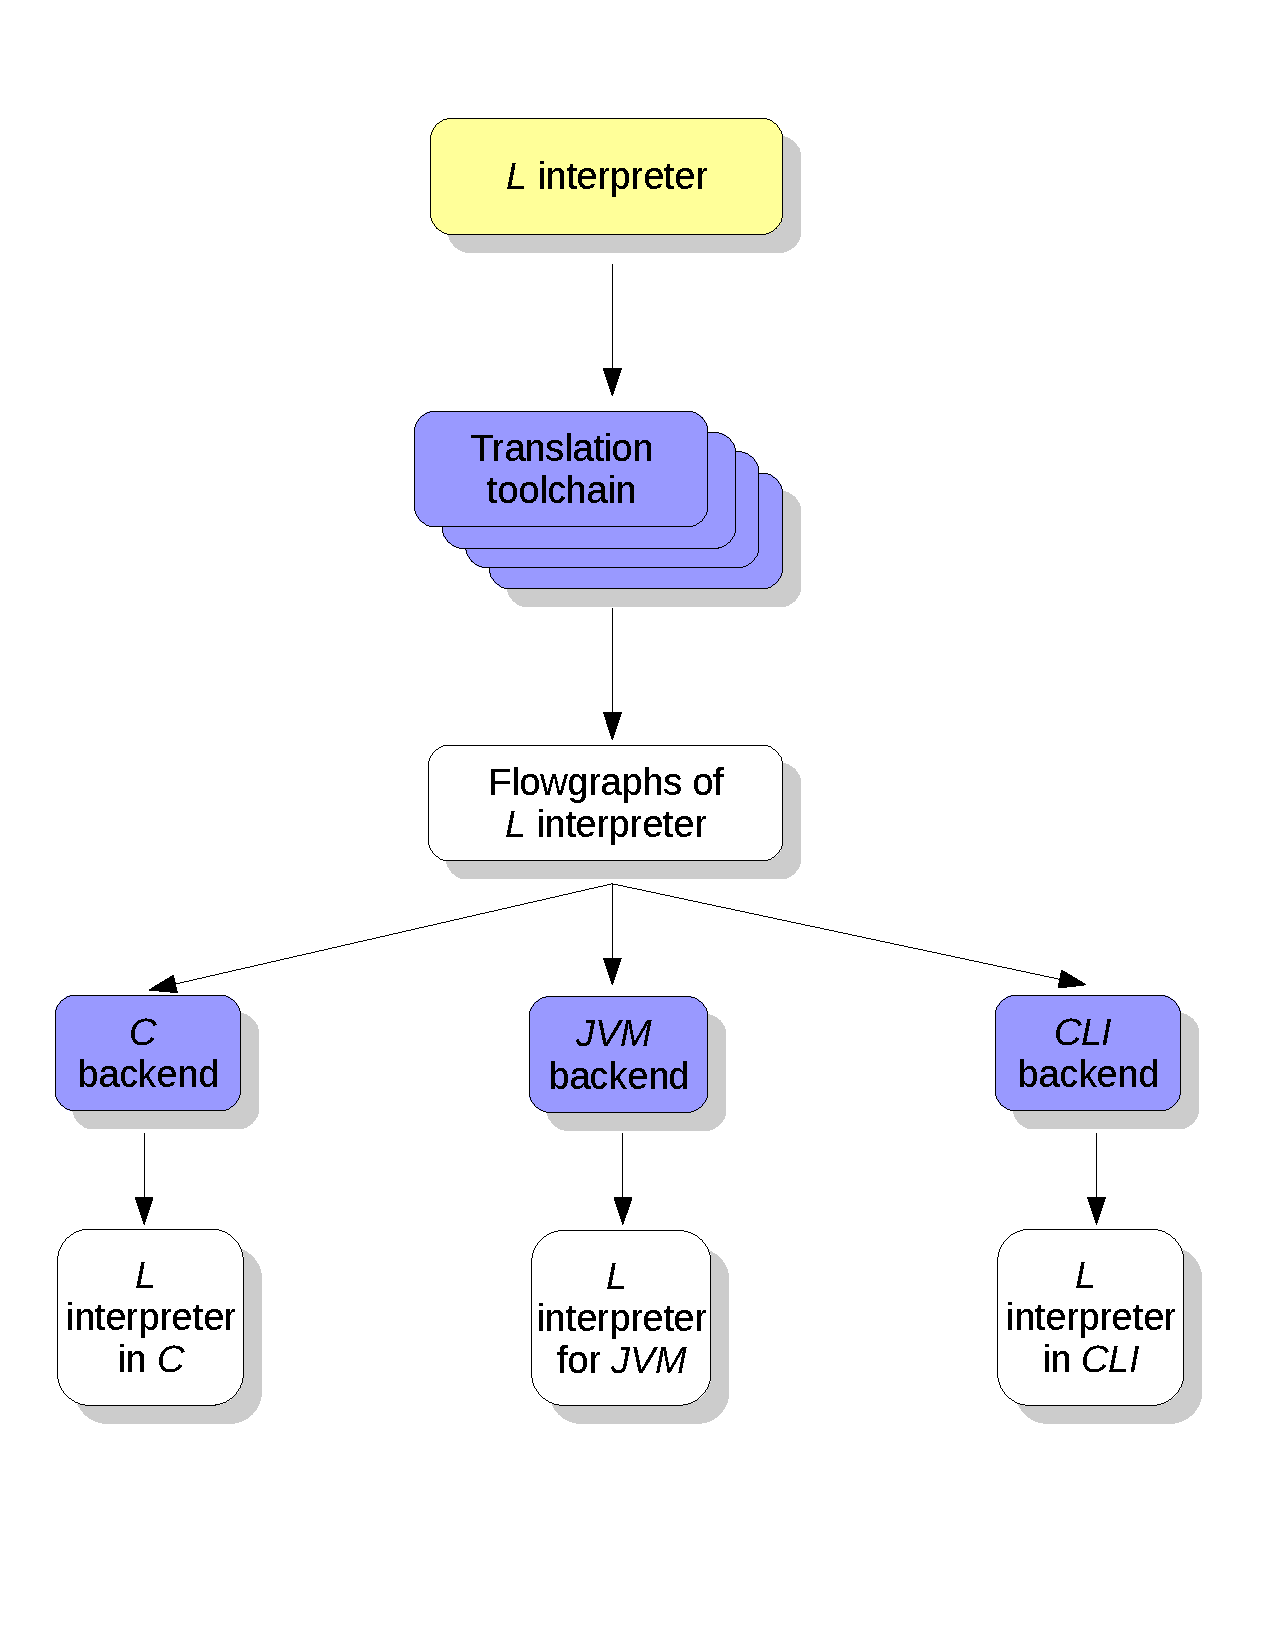
\includegraphics[width=.6\textwidth]{diagram0}
\caption{PyPy infrastracture for generating an interpreter of a
  language $L$ for several platforms}\label{pypy-fig}
\end{center}
\end{figure}
}

The \emph{PyPy} project\footnote{\texttt{http://codespeak.net/pypy/}}
\cite{RigoPedroni06} was initially conceived to develop an implementation of Python which
could be easily portable and extensible without renouncing efficiency.
To achieve these aims, the PyPy implementation is based on a highly
modular design which allows high-level aspects
to be separated from lower-level implementation details.
The abstract semantics of Python is defined by an interpreter written
in a high-level language, called RPython \cite{AACM-DLS07}, which is in fact a subset of
Python where some dynamic features have been sacrificed to allow an
efficient translation of the interpreter to low-level code.

Compilation of the interpreter is implemented as a stepwise
refinement by means of a translation toolchain which performs type
analysis, code optimizations and several transformations aiming at 
incrementally providing implementation details such as memory management or the threading model.
The different kinds of intermediate codes  which are refined 
during the translation process are all represented by a collection of control flow graphs,
at several levels of abstractions.

Finally, the low-level control flow-graphs produced by the toolchain
can be translated to executable code for a specific platform by a
corresponding backend.
Currently, three fully developed backends are available to produce
executable C/POSIX code, Java and CLI/.NET bytecode. 

Despite having been specifically developed for Python, the PyPy infrastructure
can in fact be used for implementing other languages. Indeed, there were
successful experiments of using PyPy to implement several other languages such
as Smalltalk \cite{BolzEtAl08}, JavaScript, Scheme and Prolog.

\commentout{
As suggested by Figure~\ref{pypy-fig}, a portable interpreter for a
generic language $L$  can be
easily developed once an interpreter for $L$ has been implemented in
RPython.
}

\subsection{PyPy and JIT-Generation}

One of the most important aspects that PyPy's translation toolchain can weave
in is the \emph{automatic generation of a JIT compiler}.  This section will
give a high-level overview of how the JIT-generation process works. More
details will be given in subsequent sections.

The first step is to write an interpreter for the chosen language.  Since it
must be fed to the translation toolchain, the interpreter has to be written in
RPython.  Then, to guide the process, we need to add few manual
annotations to the interpreter, in order to teach the JIT generator which
informations are important to know at compile-time.  Annotations are inserted
as \emph{hints}, as described in section \ref{sec:hints}.

It is important to distinguish between three distinct phases of execution:

\begin{enumerate}
\item \textbf{Translation-time}: when the translation toolchain runs and the
  JIT compiler is automatically generated from the interpreter.  The result is
  an executable that can be used to run programs written in the chosen
  language.
\item \textbf{Compile-time}: when the JIT compiler runs, generating executable
  code on the fly.
\item \textbf{Runtime}: when the code generated at compile-time is executed.
\end{enumerate}

Note that in this schema translation-time happens only once, on the
developer's machine.  By contrast, compile-time and runtime happens every time
the user wants to run some program.

Generating efficient compilers for dynamic languages is hard.  Since these
languages are dynamically typed, usually the compiler does not have enough
information to produce efficient code, but instead it has to insert a lot of
runtime checks to select the appropriate implementation for each operation.

By emitting code at runtime, JIT compilers can exploit some extra knowledge
compared to traditional static compilers.  However, we need to take special
care to choose a strategy for JIT compilation that lets the compiler to take
the best of this advantage.

Most JIT compilers for dynamic languages around (such as
IronPython\footnote{http://www.codeplex.com/IronPython},
Jython\footnote{http://www.jython.org/} or
JRuby\footnote{http://jruby.codehaus.org/}) compile code at the method
granularity.  If on the one hand they can exploit some of the knowledge
gathered at runtime (e.g. the types of method parameters), on the other hand
they can do little to optimize most of the operations inside, because few
assumptions can be made about the global state of the program.

JIT compilers generated by PyPy solve this problem by delaying the compilation
until they know all the informations needed to generate efficient code.  If at
some point the JIT compiler does not know about something it needs, it
generates a callback into itself and stops execution.  

Later, when the generated code is executed, the callback might be hit and the JIT
compiler is restarted again.  At this point, the JIT knows exactly the state
of the program and can exploit all this extra knowledge to generate highly
efficient code.  Finally, the old code is patched and linked to the newly
generated code, so that the next time the JIT compiler will not be invoked
again.  As a result, \textbf{runtime and compile-time are continuously
interleaved}. The primitive to do this sort of interleaving is called promotion,
it is described in Section \ref{sec:promotion}.

One of the most important optimizations that the generated JIT does is removing
unnecessary allocations. This is described in Section \ref{sec:virtuals}

Modifying the old code to link to the newly generated one is very challenging on
.NET, as the framework does not offer any primitive to do this.  Section
\ref{sec:clibackend} explains how it is possible to simulate this behaviour.

\section{The TLC language}

In this section, we will briefly describe \emph{TLC}, a simple dynamic
language that we developed to exercise our JIT compiler generator and that will
be used as a running example in this paper. The design goal of the language is
to be very simple (the interpreter of the full language consists of about 600
lines of RPython code) but to still have the typical properties of dynamic
languages that make them hard to compile. \emph{TLC} is implemented with a small
interpreter that interprets a custom bytecode instruction set. Since our main
interest is in the runtime performance of the interpreter, we did not implement
the parser nor the bytecode compiler, but only the interpreter itself.

TLC provides four different types:
\begin{enumerate}
\item Integers
\item \lstinline{nil}, whose only value is the null value
\item Objects
\item Lisp-like lists
\end{enumerate}

Objects represent a collection of named attributes (much like JavaScript or
Self) and named methods.  At creation time, it is necessary to specify the set
of attributes of the object, as well as its methods.  Once the object has been
created, it is possible to call methods and read or write attributes, but not
to add or remove them.

The interpreter for the language is stack-based and uses bytecode to represent
the program. It provides the following bytecode instructions:

\begin{itemize}
\item \textbf{Stack manipulation}: standard operations to manipulate the
  stack, such as \lstinline{POP}, \lstinline{PUSHARG}, \lstinline{SWAP}, etc.
\item \textbf{Flow control} to do conditional (\lstinline{BR_COND}) and
  unconditional (\lstinline{BR}) jumps.
\item \textbf{Arithmetic}: numerical operations on integers, like
  \lstinline{ADD}, \lstinline{SUB}, etc.
\item \textbf{Comparisons} like \lstinline{EQ}, \lstinline{LT},
  \lstinline{GT}, etc.
\item \textbf{Object-oriented} operations: \lstinline{NEW},
  \lstinline{GETATTR}, \lstinline{SETATTR}, \lstinline{SEND}.
\item \textbf{List operations}: \lstinline{CONS}, \lstinline{CAR},
  \lstinline{CDR}.
\end{itemize}

Obviously, not all the operations are applicable to all types. For example,
it is not possible to \lstinline{ADD} an integer and an object, or reading an
attribute from an object which does not provide it.  Being dynamically typed,
the interpreter needs to do all these checks at runtime; in case one of the check
fails, the execution is simply aborted.

\subsection{TLC properties}
\label{sec:tlc-properties}

Despite being very simple and minimalistic, \lstinline{TLC} is a good
candidate as a language to test our JIT generator, as it has some of the
properties that makes most of current dynamic languages so slow:

\begin{itemize}

\item \textbf{Stack based interpreter}: this kind of interpreter requires all the operands to be
  on top of the evaluation stack.  As a consequence programs spend a lot of
  time pushing and popping values to/from the stack, or doing other stack
  related operations.  However, thanks to its simplicity this is still the
  most common and preferred way to implement interpreters.

\item \textbf{Boxed integers}: integer objects are internally represented as
  an instance of the \lstinline{IntObj} class, whose field \lstinline{value}
  contains the real value.  By having boxed integers, common arithmetic
  operations are made very slow, because each time we want to load/store their
  value we need to go through an extra level of indirection.  Moreover, in
  case of a complex expression, it is necessary to create many temporary
  objects to hold intermediate results.

\item \textbf{Dynamic lookup}: attributes and methods are looked up at
  runtime, because there is no way to know in advance if and where an object
  have that particular attribute or method.
\end{itemize}


\subsection{TLC example}

As we said above, TLC exists only at bytecode level; to ease the development
of TLC programs, we wrote an assembler that generates TLC bytecode. Figure \ref{fig:tlc-abs}
shows a simple program that computes the absolute value of
the given integer.  In the subsequent sections, we will examine step-by-step 
how the generated JIT compiler manages to produce a fully optimized version of it.

\begin{figure}[h]
\begin{center}
\begin{lstlisting}
main:             # stack: []
    PUSHARG       #        [n]
    PUSH 0        #        [n, 0]
    LT            #        [0 or 1]
    BR_COND neg

pos:              #        []
    PUSHARG       #        [n]
    RETURN

neg:
    PUSH 0        #        [0]
    PUSHARG       #        [0,n]
    SUB           #        [-n]
    RETURN
\end{lstlisting}
\caption{The TLC bytecode for computing the absolute value of a function}
\label{fig:tlc-abs}
\end{center}
\end{figure}

\section{Automatic generation of JIT compilers}

Traditional JIT compilers are hard to write, time consuming and hard to
evolve.  On the other hand, interpreters are easy both to write and maintain,
but they are usually slow.  By automatically generating a JIT compiler out of
an interpreter, we take the best of both worlds.

\commentout{
\begin{figure}[h]
\begin{center}
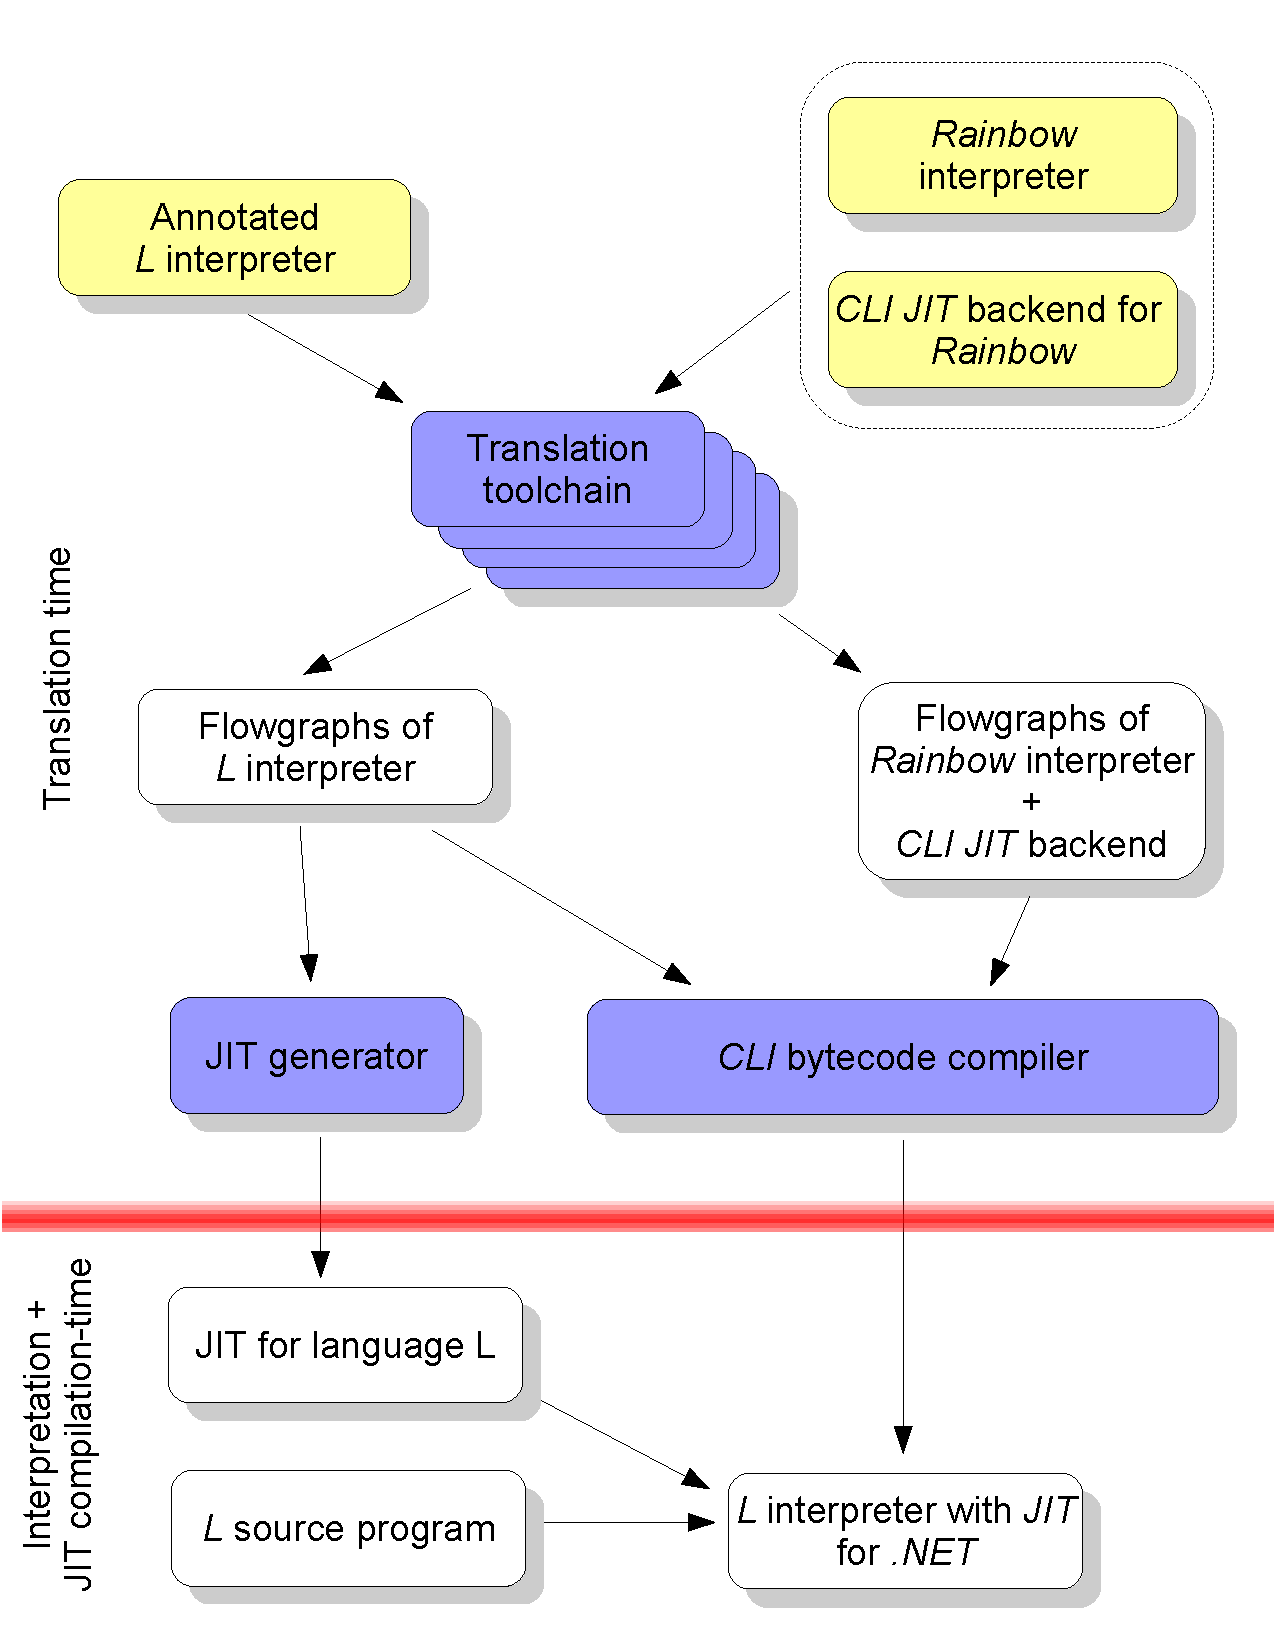
\includegraphics[width=.6\textwidth]{diagram1}
\caption{PyPy infrastructure for generating an interpreter of a
  language $L$ with JIT compilation for the .NET platform}
\end{center}
\end{figure}
}

The JIT generation framework uses partial evaluation techniques to generate a
dynamic compiler from an interpreter; the idea is inspired by Psyco \cite{DBLP:conf/pepm/Rigo04}, which
uses the same techniques but it's manually written instead of being
automatically generated.

\subsection{Partial evaluation}

Yoshihiko Futamura published a paper \cite{Futamura99} that proposed a
technique to automatically transform an interpreter of a programming language
into a compiler for the same language. This would solve the problem of having to
write a compiler instead of a much simpler interpreter. He proposed to use
partial evaluation to achieve this goal. He defined partial evaluation along the following lines:

Given a program $P$ with $m + n$ input variables $s_1, ..., s_m$ and $d_1, ...,
d_n$, the partial evaluation of $P$ with respect to concrete values $s'_1, ...,
s'_m$ for the first $m$ variables is a program $P'$. The program $P'$ takes only
the input variables $d_1, ..., d_n$ but behaves exactly like $P$ with the
concrete values (but is hopefully more efficient). This transformation is done
by a program $S$, the partial evaluator, which takes $P$ and $s_1, ..., s_m$ as
input:

    $$S(P, (s'_1, ..., s'_m)) = P'$$

The variables $s_1, ..., s_m$ are called the \emph{static} variables, the
variables $d_1, ..., d_n$ are called the \emph{dynamic} variables; $P'$ is the
\emph{residual code}. Partial evaluation creates a version of $P$ that works
only for a fixed set of inputs for the first $m$ arguments. This effect is
called \emph{specialization}.

When $P$ is an interpreter for a programming language, then the $s_1, ..., s_m$
are chosen such that they represent the program that the interpreter is
interpreting and the $d_1, ..., d_n$ represent the input of this program. Then
$P'$ can be regarded as a compiled version of the program that the chosen $s'_1,
..., s'_m$ represent, since it is a version of the interpreter that can only
interpret this program. Now once the partial evaluator $S$ is implemented, it is
actually enough to implement an interpreter for a new language and use $S$
together with this interpreter to compile programs in that new language.

A valid implementation for $S$ would be to just put the concrete values into $P$
to get $P'$, which would not actually produce any performance benefits compared with
directly using $P$. A good implementation for $S$ should instead make use of the
information it has and evaluate all the parts of the program that actually
depend only on the $s_1, ..., s_m$ and to remove parts of $P$ that cannot be
reached given the concrete values.

\begin{figure}[h]
\begin{center}
\input{tlc-simplified.py}
\caption{The main loop of the TLC interpreter, written in RPython}
\label{fig:tlc-main}
\end{center}
\end{figure}

Let us look at an example. Figure \ref{fig:tlc-main} shows parts of the
main-loop of the TLC interpreter (in slightly simplified form). The static
arguments of this functions would typically be the \lstinline{code} argument
(containing the bytecode as a string), the \lstinline{pc} argument (containing
the initial program counter) and the \lstinline{pool} argument (containing the
constant pool). The \lstinline{args} argument is dynamic since it contains the
user-input of the interpreted function. Since the \lstinline{while} loop and the
contained conditions depend only on static arguments it will typically be
unrolled by a partial evaluator.

When the function is partially evaluated with respect to the TLC example
function shown in Figure \ref{fig:tlc-abs} (which computes the absolute value of a number),
the residual code would look like in Figure \ref{fig:tlc-folded}. This version
is already a great improvement over pure interpretation, all the bytecode
dispatch overhead has been removed. However, the function as shown is still
rather inefficient, due to lots of superfluous stack handling and also due to
some indirect calls for implementing comparison (\lstinline{lt}) and
subtraction (\lstinline{sub}).

\begin{figure}[h]
\begin{center}
\input{tlc-folded.py}
\caption{The residual code of the TLC main loop with respect to the
\lstinline{abs} function }
\label{fig:tlc-folded}
\end{center}
\end{figure}

This shows a common shortcoming of partial evaluation when applied to a dynamic
language: The partial evaluator (just like an ahead-of-time compiler) cannot
make assumptions about the types of objects, which leads to poor results.
Effective dynamic compilation requires feedback of runtime information into
compile-time. This is no different for partial evaluation, and subsequent sections shows how we managed to solve this problem.


\subsection{Binding Time Analysis in PyPy}

At translation time, PyPy performs binding-time analysis of the source RPython
program, to determine which variables are static and which dynamic.  The
binding-time terminology that we are using in PyPy is based on the colors that
we use when displaying the control flow graphs:

\begin{itemize}
\item \emph{Green} variables contain values that are known at compile-time.
They correspond to static arguments.
\item \emph{Red} variables contain values that are usually not known
compile-time. They correspond to dynamic arguments.
\end{itemize}

The binding-time analyzer of our translation tool-chain is using a simple
abstract-interpretation based analysis. It is based on the
same type inference engine that is used on the source RPython program.
This is called the \emph{hint-annotator}; it
operates over input flowgraphs
and propagates annotations that do not track types but
value dependencies and manually-provided binding time hints.

The normal process of the hint-annotator is to propagate the binding
time (i.e. color) of the variables using the following kind of rules:

\begin{itemize}
\item For a foldable operation (i.e. one without side effect and which depends
only on its argument values), if all arguments are green, then the result can
be green too.

\item Non-foldable operations always produce a red result.

\item At join points, where multiple possible values (depending on control
flow) are meeting into a fresh variable, if any incoming value comes from a red
variable, the result is red.  Otherwise, the color of the result might be
green.  We do not make it eagerly green, because of the control flow
dependency: the residual function is basically a constant-folded copy of the
source function, so it might retain some of the same control flow.  The value
that needs to be stored in the fresh join variable thus depends on which
branches are taken in the residual graph.
\end{itemize}

\subsection{Hints}
\label{sec:hints}

Our goal in designing our approach to binding-time analysis was to
minimize the number of explicit hints that the user must provide in
the source of the RPython program.  This minimalism was not pushed to
extremes, though, to keep the hint-annotator reasonably simple.  

The driving idea was that hints should be need-oriented.  Indeed, in a
program like an interpreter, there are a small number of places where it
would be clearly beneficial for a given value to be known at
compile-time, i.e. green: this is where we require the hints to be
added.

The hint-annotator assumes that all variables are red by default, and
then propagates annotations that record dependency information.
When encountering the user-provided hints, the dependency information
is used to make some variables green.  All
hints are in the form of an operation \texttt{hint(v1, someflag=True)}
which semantically just returns its first argument unmodified.

The crucial need-oriented hint is \texttt{v2 = hint(v1, concrete=True)}
which should be used in places where the programmer considers the
knowledge of the value to be essential.  This hint is interpreted by
the hint-annotator as a request for both \texttt{v1} and \texttt{v2} to be green.  It
has a \emph{global} effect on the binding times: it means that not only
\texttt{v1} but all the values that \texttt{v1} depends on – recursively –
are forced to be green.  The hint-annotator gives an error if the
dependencies of \texttt{v1} include a value that cannot be green, like
a value read out of a field of a non-immutable instance.

Such a need-oriented backward propagation has advantages over the
commonly used forward propagation, in which a variable is compile-time
if and only if all the variables it depends on are also compile-time.  A
known issue with forward propagation is that it may mark as compile-time
either more variables than expected (which leads to over-specialization
of the residual code), or less variables than expected (preventing
specialization to occur where it would be the most useful).  Our
need-oriented approach reduces the problem of over-specialization, and
it prevents under-specialization: an unsatisfiable \texttt{hint(v1,
concrete=True)} is reported as an error.

There are cases in which having a green variable is essential for generating
good code, but it is not possible to use the \texttt{concrete} hint due to an
unsatisfiable dependency: Section~\ref{sec:promotion} introduces
\emph{promotion}, the novel technique that makes possible to solve this
problem.

\section{Automatic Unboxing of Intermediate Results}
\label{sec:virtuals}

Interpreters for dynamic languages typically continuously allocate a lot of small
objects, for example due to boxing. This makes arithmetic operations extremely
inefficient. For this reason, we
implemented a way for the compiler to try to avoid memory allocations in the
residual code as long as possible. The idea is to try to keep new
run-time instances \emph{exploded}: instead of a single run-time object allocated on
the heap, the object is \emph{virtualized} as a set
of fresh local variables, one per field. Only when the object can be accessed by from
somewhere else is it actually allocated on the heap. The effect of this is similar to that of
escape analysis \cite{Blanchet99escapeanalysis}, \cite{Choi99escapeanalysis},
which also prevents allocations of objects that can be proven to not escape a
method or set of methods (the algorithms however are a lot more advanced than
our very simple analysis).

It is not always possible to keep instances virtual.  The main
situation in which it needs to be \emph{forced} (i.e. actually allocated at
run-time) is when the pointer escapes to some non-virtual location like
a field of a real heap structure.  Virtual instances still avoid the run-time
 allocation of most short-lived objects, even in non-trivial situations.  

In addition to virtual instances, the compiler can also handle virtual
containers, namely lists and dictionaries\footnote{(R)Python's dictionaries
  are equivalent to .NET \lstinline{Hashtable}s}.  If the indexing operations
can be evaluated at compile-time (i.e., if the variables holding the indexes
are green), the compiler internally keeps track of the state of the container
and store the items as local variables.

Look again at figure \ref{fig:tlc-folded}: the list in the \lstinline{stack}
variable never escapes from the function.  Moreover, all the indexing
operations (either done explicitly or implicitly by \lstinline{append} and
\lstinline{pop}) are evaluable at compile-time.  Thus, the list is kept
\emph{virtual} and its elements are stored in variables $v_n$, where $n$
represents the index in the list.  Figure \ref{fig:tlc-folded-virtualized}
show how the resulting code looks like; to ease the reading, the state of the
\lstinline{stack} as kept by the compiler is shown in the comments.

\begin{figure}[h]
\begin{center}
\input{tlc-folded-virtualized.py}
\caption{The result of virtualizing the \lstinline{stack} list}
\label{fig:tlc-folded-virtualized}
\end{center}
\end{figure}

Even if not shown in the example, \lstinline{stack} is not the only
virtualized object.  In particular the two objects created by
\lstinline{IntObj(0)} are also virtualized, and their fields are stored as
local variables as well.  Virtualizion of instances is important not only
because it avoids the allocation of unneeded temporary objects, but also
because it makes possible to optimize method calls on them, as the JIT
compiler knows their exact type in advance.


\section{Promotion}
\label{sec:promotion}

In the sequel, we describe in more details one of the main new
techniques introduced in our approach, which we call \emph{promotion}.  In
short, it allows an arbitrary run-time (i.e. red) value to be turned into a
compile-time (i.e. green) value at any point in time.  Promotion is thus the central way by
which we make use of the fact that the JIT is running interleaved with actual
program execution. Each promotion point is explicitly defined with a hint that
must be put in the source code of the interpreter.

From a partial evaluation point of view, promotion is the converse of
the operation generally known as \emph{lift}.  Lifting a value means
copying a variable whose binding time is compile-time into a variable
whose binding time is run-time – it corresponds to the compiler
``forgetting'' a particular value that it knew about.  By contrast,
promotion is a way for the compiler to gain \emph{more} information about
the run-time execution of a program. Clearly, this requires
fine-grained feedback from run-time to compile-time, thus a
dynamic setting.

Promotion requires interleaving compile-time and run-time phases,
otherwise the compiler can only use information that is known ahead of
time. It is impossible in the ``classical'' approaches to partial
evaluation, in which the compiler always runs fully ahead of execution.
This is a problem in many realistic use cases.  For example, in an
interpreter for a dynamic language, there is mostly no information
that can be clearly and statically used by the compiler before any
code has run.

A very different point of view on promotion is as a generalization of
techniques that already exist in dynamic compilers as found in modern virtual
machines for object-oriented language, like \emph{Polymorphic Inline Cache}
(PIC, \cite{hoelzle_optimizing_1991}) and its variations, whose main goal is
to optimize and reduce the overhead of dynamic dispatching and indirect
invocation: the dynamic lookups are cached and the corresponding generated
machine code contains chains of compare-and-jump instructions which are
modified at run-time.  These techniques also allow the gathering of
information to direct inlining for even better optimization results. Compared
to PICs, promotion is more general because it can be applied not only to
indirect calls but to any kind of value, including instances of user-defined
classes or integer numbers.

In the presence of promotion, dispatch optimization can usually be
reframed as a partial evaluation task.  Indeed, if the type of the
object being dispatched to is known at compile-time, the lookup can be
folded, and only a (possibly even inlined) direct call remains in the
generated code.  In the case where the type of the object is not known
at compile-time, it can first be read at run-time out of the object and
promoted to compile-time.  As we will see in the sequel, this produces
machine code very similar to that of polymorphic inline
caches.

The essential advantage of promotion is that it is no longer tied to the details of
the dispatch semantics of the language being interpreted, but applies in
more general situations.  Promotion is thus the central enabling
primitive to make partial evaluation a practical approach to language
independent dynamic compiler generation.

Promotion is invoked with the use of a hint as well:
\lstinline{v2 = hint(v1, promote=True)}.
This hint is a \emph{local} request for \texttt{v2} to be green, without
requiring \texttt{v1} to be green.  Note that this amounts to copying
a red value into a green one, which is not possible in classical
approaches to partial evaluation. A slightly different hint can be used to
promote the \emph{class} of an instance. This is done with
\lstinline{hint(v1, promote_class=True)}. It does not have an effect on the
bindings of any variable.


\subsection{Implementing Promotion}
\label{sec:implementing-promotion}

The implementation of promotion requires a tight coupling between
compile-time and run-time: a \emph{callback}, put in the generated code,
which can invoke the compiler again.  When the callback is actually
reached at run-time, and only then, the compiler resumes and uses the
knowledge of the actual run-time value to generate more code.

The new generated code is potentially different for each run-time value
seen.  This implies that the generated code needs to contain some sort
of updatable switch, or \emph{flexswitch}, which can pick the right code path based on the
run-time value.

Let us look again at the TLC example.  To ease the reading, figure
\ref{fig:tlc-main} showed a simplified version of TLC's main loop, which did
not include the hints.  The implementation of the \lstinline{LT} opcode with
hints added is shown in figure \ref{fig:tlc-main-hints}.

\begin{figure}[h]
\begin{center}
\begin{tabular}{l|l}
\begin{lstlisting}
def interp_eval(code, pc, args, pool):
  code_len = len(code)
  stack = []
  while pc < code_len:
      opcode = ord(code[pc])
      opcode = hint(opcode, concrete=True)
      pc += 1

      if opcode == PUSH:
          ...
      elif opcode == LT:
        a, b = stack.pop(), stack.pop()
        hint(a, promote_class=True)
        hint(b, promote_class=True)
        stack.append(IntObj(b.lt(a)))
\end{lstlisting}
&
\hspace{2pt}
\begin{lstlisting}
class IntObj(Obj):

  def lt(self, other): 
    return (self.value < 
            other.int_o())

  def sub(self, other):
    return IntObj(self.value -
                  other.int_o())

  def int_o(self):
    return self.value

  ...
\end{lstlisting}
\end{tabular}
\end{center}
\caption{Usage of hints in TLC's main loop and excerpt of the \lstinline{IntObj} class}
\label{fig:tlc-main-hints}
\end{figure}

By promoting the class of \lstinline{a} and \lstinline{b}, we tell the JIT
compiler not to generate code until it knows the exact RPython class of both.
Figure \ref{fig:tlc-abs-promotion-1} shows the
code\footnote{\lstinline{switch} is not a legal (R)Python statement, it is
  used here only as a pseudocode example.} generated while compiling the usual
\lstinline{abs} function: note that, compared to figure
\ref{fig:tlc-folded-virtualized}, the code stops just before the call
\lstinline{b.lt(a)}.

\begin{figure}[h]
\begin{center}
\begin{lstlisting}[language=Python]
def interp_eval_abs(args):
    v0 = args[0]
    v1 = IntObj(0)
    a, b = v0, v1
    # hint(a, promote_class=True) implemented as follows:
    cls_a = a.__class__
    switch cls_a:
        default: 
            continue_compilation(jitstate, cls_a)
\end{lstlisting}
\caption{Promotion step 1}
\label{fig:tlc-abs-promotion-1}
\end{center}
\end{figure}

\begin{figure}[h]
\begin{center}
\begin{lstlisting}[language=Python]
def interp_eval_abs(args):
    v0 = args[0]
    v1 = IntObj(0)
    a, b = v0, v1
    # hint(a, promote_class=True) implemented as follows:
    cls_a = a.__class__
    switch cls_a:
        IntObj:
            # hint(b, promote_class=True) needs no code
            v0 = IntObj(b.value < a.value)
            cond = v0
            if cond.value:
                return a
            else:
                v0 = IntObj(0)
                v1 = args[0]
                a, b = v0, v1
                v0 = IntObj(b.value - a.value)
                return v0
        default: 
            continue_compilation(jitstate, cls_a)
\end{lstlisting}
\caption{Promotion step 2}
\label{fig:tlc-abs-promotion-2}
\end{center}
\end{figure}

The first time the flexswitch is executed, the \lstinline{default} branch is
taken, and the special function \lstinline{continue_compilation} restarts the
JIT compiler, passing it the just-seen value of \lstinline{cls_a}.  The JIT
compiler generates new specialized code, and \emph{patches} the flexswitch to
add the new case, which is then executed.

If later an instance of \lstinline{IntObj} hits the flexswitch again, the
code is executed without needing more calls to the JIT compiler.  On the
other hand, if the flexswitch is hit by an instance of some other class, the
\lstinline{default} branch will be selected again and the whole process will
restart.

Now, let us examine the content of the \lstinline{IntObj} case: first, there
is a hint to promote the class of \lstinline{b}.  Although in general
promotion is implemented through a flexswitch, in this case it is not needed
as \lstinline{b} holds a \emph{virtual instance}, whose class is already
known (as described in the previous section).

Then, the compiler knows the exact class of \lstinline{b}, thus it can inline
the calls to \lstinline{lt}.  Moreover, inside \lstinline{lt} there is a
call to \lstinline{a.int_o()}, which is inlined as well for the very same
reason.  Moreover, as we saw in section \ref{sec:virtuals}, the \lstinline{IntObj}
instance can be virtualized, so that the subsequent \lstinline{BR_COND} opcode
can be compiled efficiently without needing any more flexswitch.

Figure~\ref{fig:tlc-abs-final} shows the final, fully optimized version of the
code, with all the instances virtualized and the unneeded temporary variables
removed.

\begin{figure}[h]
\begin{center}
\begin{lstlisting}[language=Python]
def interp_eval_abs(args):
    a = args[0]
    cls_a = a.__class__
    switch cls_a:
        IntObj:
            # 0 is the constant "value" field of the virtualized IntObj(0)
            if 0 < a.value:
                return a
            else:
                return IntObj(0 - a.value)
        default: 
            continue_compilation(jitstate, cls_a)
\end{lstlisting}
\caption{Final optimized version of the \lstinline{abs} example}
\label{fig:tlc-abs-final}
\end{center}
\end{figure}

\section{The CLI JIT backend}
\label{sec:clibackend}

\subsection{JIT layering}

From the implementation point of view, the JIT generator is divided into a
frontend and several backends.  The goal of the frontend is to generate a JIT
compiler which works as described in the previous sections.  Internally, the
JIT represents the compiled code as \emph{flow graphs}, and the role of
the backends is to translate flowgraphs into machine code.

At the moment of writing, three backends have been implemented: one for Intel
\emph{x86} processors, one for \emph{PowerPC} processors, and one for the
\emph{CLI Virtual Machine}.  The latter is special because instead of emitting
code for a real CPU it emits code for a virtual machine\footnote{By using the 
\lstinline{Reflection.Emit} namespace and creating \lstinline{DynamicMethod}s.}: 
before being executed, the generated code will be compiled again by the .NET JIT
compiler.

Thus, when using the CLI backend, we actually have two JIT compilers at two different
layers, each one specialized in different kinds of optimization.
By operating at a higher level, our JIT can potentially do a better job 
in some contexts, as our benchmarks demonstrate (see
Section~\ref{sec:benchmarks}).  On the other hand, the lower-level .NET JIT is
very good at producing machine code, much more than PyPy's own \emph{x86}
backend, for example.  By combining the strengths of both we can get highly
efficient machine code.

As usual, the drawback is that programs that runs for a very short period of
time could run slower with JIT than without, due to the time spent doing the
initial (double) compilation.  
Finally, it is important to underline that while we have directed our efforts 
to generate a JIT compiler able to emit very efficient code,
the performance of the compiler itself has been neglected so far, but  
it is certainly an issue which will have to be considered in our future research.

\subsection{Flexswitches}

For a large part, implementing the CLI backend is easy and straightforward, as
there is a close correspondence between most of the operations used by
frontend's flowgraphs and the CLI instructions.  Thus, we will not go into
details for this part.

However the concept of \emph{flexswitch}, as described in
Section~\ref{sec:jitgen}, does not have any direct equivalent
in the CLI model, and it is hard to implement efficiently.

A flexswitch is a special kind of switch which can be dynamically
extended with new cases.  Intuitively, its behavior can be described
well in terms of flow graphs: a flexswitch can be considered 
as a special flow graph block where links to newly created blocks are
dynamically added whenever new cases are needed. 

\begin{figure}[h]
\begin{center}
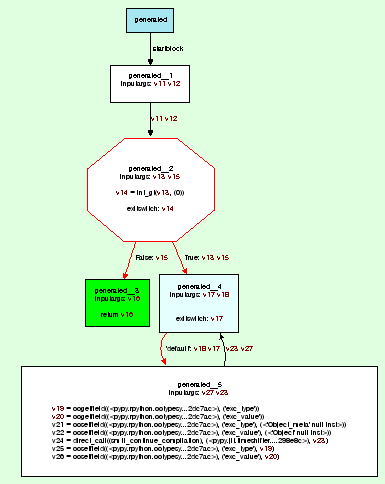
\includegraphics[height=5cm]{flexswitch1}
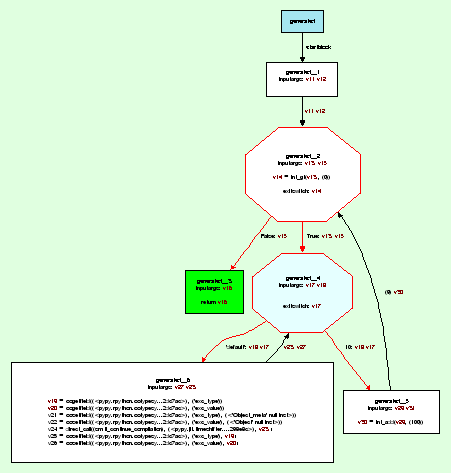
\includegraphics[height=5cm]{flexswitch2}
\caption{An example of a flexswitch evolution: in the picture on the
  right block D has been dynamically added.}\label{flexswitch-fig}
\end{center}
\end{figure}

In the pictures of Figure~\ref{flexswitch-fig}, block B (highlighted in grey)
corresponds to a flexswitch; initially (picture on the left) 
only block C, containing the code to restart the JIT compilation,
is connected to the flexswitch; the picture on the right
shows the graph after the first case has been dynamically added to the flexswitch,
by linking block B with the freshly created block D.


\subsection{Implementing flexswitches in CLI}
\label{sec:flexswitches-cli}

Implementing flexswitches for backends generating machine code is
not too complex: basically, a new jump has to be inserted in the
existing code to point to the newly generated code fragment.

Unfortunately, CLI does not allow modification of code which
has been already loaded and linked, therefore the simplest approach
taken for low level architectures does not work.

Since in .NET methods are the basic units of compilation, a possible
solution consists in creating a new method 
any time a new case has to be added to a flexswitch.

It is important to underline the difference between flow graphs and methods:
the first are the logical unit of code as seen by the JIT compiler, each of
them being concretely implemented by \emph{one or more} methods.

In this way, whereas flow graphs without flexswitches are translated to a
single method, the translation of \emph{growable} flow graphs will be
scattered over several methods.  Summarizing, the backend behaves in the
following way:
\begin{itemize}
\item Each flow graph is translated in a collection of methods which
  can grow dynamically. Each collection contains at least one
  method, called \emph{primary}, which is the first to be created.
  All other methods, called \emph{secondary}, are added dynamically 
  whenever a new case is added to a flexswitch.

\item Each either primary or secondary method implements a certain
  number of blocks, all belonging to the same flow graph.
\end{itemize} 

When a new case is added to a flexswitch, the backend generates the new blocks
into a new single method.  The newly created method is pointed to by a
delegate\footnote{\emph{Delegates} are the .NET equivalent of function
  pointers.} stored in the flexswitch, so that it can be invoked later when
needed.

\subsubsection{Internal and external links}

A link is called \emph{internal} if it connects two blocks implemented
by the same method,
\emph{external} otherwise.

Following an internal link is easy in IL bytecode: a jump to
the corresponding code fragment in the same method can be emitted 
to execute the new block, whereas the appropriate local variables can be
used for passing arguments. 

Following an external link whose target is an initial block could also
be easily implemented, by just invoking the corresponding method.
What cannot be easily implemented in CLI is following an external link
whose target is not an initial block; consider, for instance, the
outgoing link from block D to block A in Figure~\ref{flexswitch-fig}. How is it possible to jump into
the middle of a method?

To solve this problem every method contains a special code, called
\emph{dispatcher}: whenever a method is invoked, its dispatcher is
executed first\footnote{The dispatcher should not be
confused with the initial block of a method.} to
determine which block has to be executed.
This is done by passing to the method a 32 bits number, called 
\emph{block id}, which uniquely identifies the next block of the graph to be executed.
The high 2 bytes of a block id constitute the \emph{method id}, which 
univocally identifies a method in a graph, whereas the low 2 bytes constitute
a progressive number univocally identifying a block inside each method.

The picture in Figure~\ref{block-id-fig} shows a graph composed of three methods (for
simplicity, dispatchers are not shown); method ids are in bold, whereas
block numbers are in black. 
The graph contains three external links; in particular, note the link
between blocks \texttt{0x00020001} and \texttt{0x00010001} which
connects two blocks implemented by different methods.
\begin{figure}[h]
\begin{center}
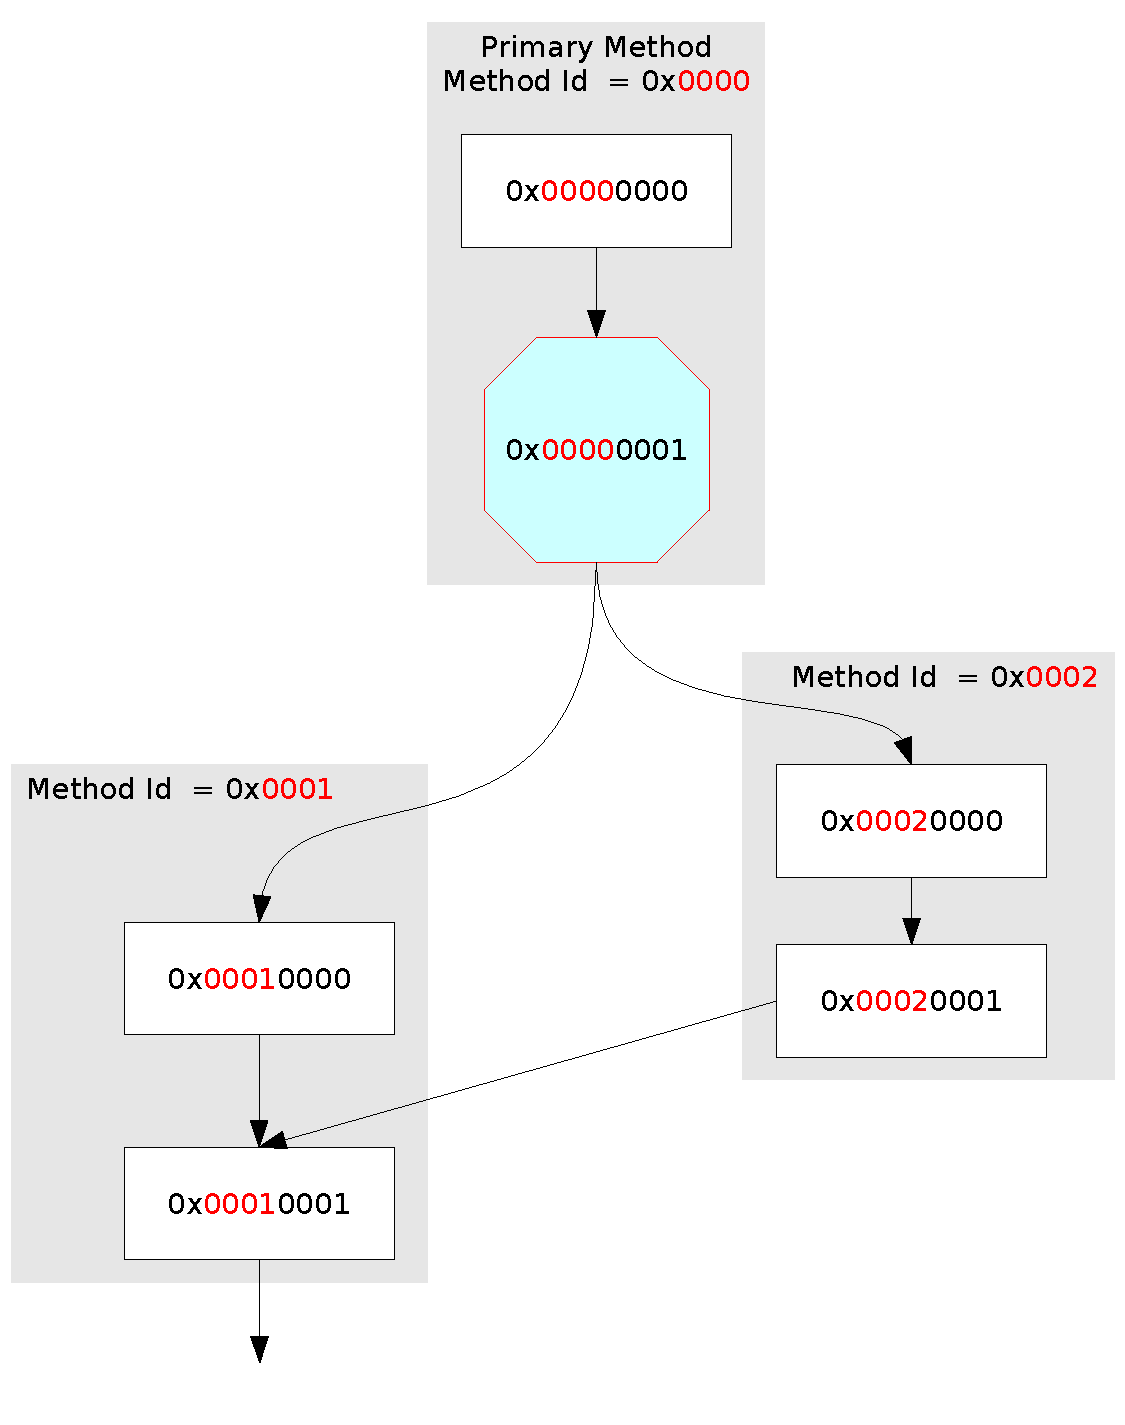
\includegraphics[height=6cm]{blockid}
\caption{Method and block ids.}\label{block-id-fig}
\end{center}
\end{figure}

The code\footnote{For simplicity we write C\# code instead of
the actual IL bytecode.} generated for the dispatcher of methods
is similar to the following fragment: 
\begin{lstlisting}[language={[Sharp]C}]
// dispatch block
int methodid = (blockid && 0xFFFF0000) >> 16; 
int blocknum = blockid && 0x0000FFFF;         
if (methodid != MY_METHOD_ID) {
  // jump_to_ext 
  ...
}
switch(blocknum) {
  case 0: goto block0;
  case 1: goto block1;
  default: throw new Exception("Invalid block id");
}
\end{lstlisting}
If the next block to be executed is implemented in the same method
(\lstinline{methodid == MY_METHOD_ID}), then the appropriate
jump to the corresponding code is executed.
Otherwise, the \lstinline{jump_to_ext}
part of the dispatcher has to be executed, which is implemented differently 
by primary and secondary methods.

The primary method is responsible for the bookkeeping of the secondary
methods which are added to the same graph dynamically. This can be 
simply implemented with an array mapping method id of secondary methods
to the corresponding delegate. Therefore, the primary methods contain
the following \lstinline{jump_to_ext} code (where
\lstinline{FlexSwitchCase} is the type of delegates for secondary methods):
\begin{lstlisting}[language={[Sharp]C}] 
// jump_to_ext
FlexSwitchCase meth = method_map[methodid];
blockid = meth(blockid, ...); // execute the method
goto dispatch_block;
\end{lstlisting}
Each secondary method returns the block id of the next block to be
executed; therefore, after the secondary method has returned, the
dispatcher of the primary method will be executed again to jump
to the correct next block. 

To avoid mutual recursion and an undesired growth of the stack,
the \lstinline{jump_to_ext} code in dispatchers of secondary methods
just returns the block id of the next block; since the primary method
is always the first method of the graph which is called, the correct
jump will be eventually executed by the dispatcher of the primary method.

Clearly this complex translation is performed only for flow graphs
having at least one flexswitch; flow graphs without flexswitches
are implemented in a more efficient and direct way by a unique method
with no dispatcher.

\subsubsection{Passing arguments to external links}

The main drawback of our solution is that passing arguments across
external links cannot be done efficiently by using the parameters of
methods for the following reasons:
\begin{itemize}
\item In general, the number and type of arguments is different for every block in a graph;

\item The number of blocks of a graph can grow dynamically, therefore
  it is not possible to compute in advance the union of the arguments
  of all blocks in a graph; 

\item Since external jumps are implemented with a delegate, all the
  secondary methods of a graph must have the same signature.
\end{itemize}

Therefore, the solution we came up with is defining a class
\lstinline{InputArgs} for passing sequences of arguments whose length
and type is variable.
\begin{lstlisting}[language={[Sharp]C}] 
public class InputArgs {
  public int[] ints;
  public float[] floats;
  public object[] objs;
  ...
}
\end{lstlisting}
Unfortunately, with this solution passing arguments to external links
becomes quite slow:
\begin{itemize}
\item When writing arguments, array re-allocation may be needed in
  case the number of arguments exceeds the dimension of the
  array. Furthermore the VM will always perform bound-checks, even
  when the size is explicitly checked in advance;

\item When reading arguments, a bound-check is performed by the VM for
  accessing each argument; furthermore, an appropriate downcast must be
  inserted anytime an argument of type object is read.
\end{itemize}
Of course, we do not need to create a new object of class
\lstinline{InputArgs} any time we need to perform an external jump;
instead, a unique object is created at the beginning of the execution
of the primary method. 

\subsubsection{Implementation of flexswitches}

To implement each flexswitch, the CLI backend creates an instance of a subclass
of \lstinline{BaseLowLevelFlexSwitch}: such an instance stores the mapping
between each value and the corresponding method we want to invoke.  Then, the
generated code contains a call to the method \lstinline{execute}, which
selects and invoke the right method depending on the actual value we are
switching on.

The following snippet shows the special case of integer flexswitches:
\begin{lstlisting}[language={[Sharp]C}] 
public class IntLowLevelFlexSwitch: 
                        BaseLowLevelFlexSwitch {
  public uint default_blockid = 0xFFFFFFFF;
  public int numcases = 0;
  public int[] values = new int[4];
  public FlexSwitchCase[] cases = 
                          new FlexSwitchCase[4];

  public void add_case(int value, FlexSwitchCase c) {
    ...
  }

  public uint execute(int value, InputArgs args) {
    for(int i=0; i<numcases; i++)
      if (values[i] == value)
        return cases[i](0, args);
    return default_blockid;
  }
}
\end{lstlisting}

The mapping from integers values to delegates (pointing to secondary
methods) is just implemented by the two arrays \lstinline{values} and
\lstinline{cases}. Method \lstinline{add_case} extends the mapping
whenever a new case is added to the flexswitch.
  
The most interesting part is the body of method \lstinline{execute},
which takes a value and a set of input arguments to be passed across
the link and jumps to the right block by performing a linear search in
array \lstinline{values}\footnote{Our microbenchmarks indicate that a linear
search is the fastest way to find the right method to call, since typically
each flexswitch contains only a very small number of cases.}.

Recall that the first argument of delegate \lstinline{FlexSwitchCase} is the
block id to jump to. By construction, the target block of a flexswitch is
always the first in a secondary method, and we use the special value
\lstinline{0} to signal this.

The value returned by method \lstinline{execute} is the next block id
to be executed; 
in case no association is found for \lstinline{value},
\lstinline{default_blockid} is returned. The value of
\lstinline{default_blockid} is initially set by the JIT compiler and
usually corresponds to a block containing code to restart the JIT
compiler for creating a new secondary method with the new code for the
missing case, and updating the flexswitch by calling method
\lstinline{add_case}.

% LocalWords:  flexswitches backend flexswitch methodid blockid xFFFF blocknum
% LocalWords:  FFFF goto FlexSwitchCase meth InputArgs ints objs VM uint args
% LocalWords:  IntLowLevelFlexSwitch BaseLowLevelFlexSwitch xFFFFFFFF numcases
% LocalWords:  JIT

\section{Benchmarks}
\label{sec:benchmarks}

In section \ref{sec:tlc-properties}, we saw that TLC provides most of the
features that usually make dynamically typed language so slow, such as
\emph{stack-based interpreter}, \emph{boxed arithmetic} and \emph{dynamic lookup} of
methods and attributes.

In the following sections, we present some benchmarks that show how our
generated JIT can handle all these features very well.

To measure the speedup we get with the JIT, we run each program three times:

\begin{enumerate}
\item By plain interpretation, without any jitting.
\item With the JIT enabled: this run includes the time spent by doing the
  compilation itself, plus the time spent by running the produced code.
\item Again with the JIT enabled, but this time the compilation has already
  been done, so we are actually measuring how good is the code we produced.
\end{enumerate}

Moreover, for each benchmark we also show the time taken by running the
equivalent program written in C\#.\footnote{The sources for both TLC and C\#
  programs are available at:

  http://codespeak.net/svn/pypy/extradoc/talk/ecoop2009/benchmarks/}

The benchmarks have been run on a machine with an Intel Pentium 4 CPU running at
3.20 GHz and 2 GB of RAM, running Microsoft Windows XP and Microsoft .NET
Framework 2.0.

\subsection{Arithmetic operations}

To benchmark arithmetic operations between integers, we wrote a simple program
that computes the factorial of a given number.  The algorithm is
straightforward, thus we are not showing the source code.  The loop contains only three operations: one
multiplication, one subtraction, and one comparison to check if we have
finished the job.

When doing plain interpretation, we need to create and destroy three temporary
objects at each iteration.  By contrast, the code generated by the JIT does
much better.  At the first iteration, the classes of the two operands of the
multiplication are promoted; then, the JIT compiler knows that both are
integers, so it can inline the code to compute the result.  Moreover, it can
\emph{virtualize} (see Section \ref{sec:virtuals}) all the temporary objects, because they never escape from
the inner loop.  The same remarks apply to the other two operations inside
the loop.

As a result, the code executed after the first iteration is close to optimal:
the intermediate values are stored as \lstinline{int} local variables, and the
multiplication, subtraction and \emph{less-than} comparison are mapped to a
single CLI opcode (\lstinline{mul}, \lstinline{sub} and \lstinline{clt},
respectively).

Similarly, we wrote a program to calculate the $n_{th}$ Fibonacci number, for
which we can do the same reasoning as above.

\begin{table}[ht]
  \begin{center}

  \begin{tabular}{l|rrrrrr}
    \multicolumn{5}{c}{\textbf{Factorial}} \\ [0.5ex]

    \textbf{$n$}          & $10$  & $10^7$           & $10^8$         & $10^9$         \\
    \hline
    \textbf{Interp}       & 0.031 & 30.984           & N/A            & N/A            \\
    \textbf{JIT}          & 0.422 &  0.453           & 0.859          & 4.844          \\
    \textbf{JIT 2}        & 0.000 &  0.047           & 0.453          & 4.641          \\
    \textbf{C\#}          & 0.000 &  0.031           & 0.359          & 3.438          \\
    \textbf{Interp/JIT 2} & N/A   & \textbf{661.000} & N/A            & N/A            \\
    \textbf{JIT 2/C\#}    & N/A   & \textbf{1.500}   & \textbf{1.261} & \textbf{1.350} \\ [3ex]


    \multicolumn{5}{c}{\textbf{Fibonacci}} \\ [0.5ex]

    \textbf{$n$}          & $10$  & $10^7$           & $10^8$         & $10^9$         \\
    \hline
    \textbf{Interp}       & 0.031 & 29.359           & 0.000          & 0.000          \\
    \textbf{JIT}          & 0.453 &  0.469           & 0.688          & 2.953          \\
    \textbf{JIT 2}        & 0.000 &  0.016           & 0.250          & 2.500          \\ 
    \textbf{C\#}          & 0.000 &  0.016           & 0.234          & 2.453          \\
    \textbf{Interp/JIT 2} & N/A   & \textbf{1879.962}& N/A            & N/A            \\
    \textbf{JIT 2/C\#}    & N/A   & \textbf{0.999}   & \textbf{1.067} & \textbf{1.019} \\
  \end{tabular}

  \end{center}
  \caption{Factorial and Fibonacci benchmarks}
  \label{tab:factorial-fibo}
\end{table}


Table \ref{tab:factorial-fibo} shows the seconds spent to calculate
the factorial and Fibonacci for various $n$.  As we can see, for small values
of $n$ the time spent running the JIT compiler is much higher than the time
spent to simply interpret the program.  This is an expected result
which, however, can be improved once we will have time
to optimize compilation and not only the generated code.

On the other, for reasonably high values of $n$ we obtain very good
results, which are valid despite the obvious overflow, since the 
same operations are performed for all experiments.
For $n$ greater than $10^7$, we did not run the interpreted program as it would have took too
much time, without adding anything to the discussion.

As we can see, the code generated by the JIT can be up to about 1800 times faster
than the non-jitted case.  Moreover, it often runs at the same speed as the
equivalent program written in C\#, being only 1.5 slower in the worst case.

The difference in speed it is probably due to both the fact that the current
CLI backend emits slightly non-optimal code and that the underyling .NET JIT
compiler is highly optimized to handle bytecode generated by C\# compilers.

As we saw in Section~\ref{sec:flexswitches-cli}, the implementation of
flexswitches on top of CLI is hard and inefficient.  However, our benchmarks
show that this inefficiency does not affect the overall performances of the
generated code.  This is because in most programs the vast majority of the
time is spent in the inner loop: the graphs are built in such a way that all
the blocks that are part of the inner loop reside in the same method, so that
all links inside are internal (and fast).


\subsection{Object-oriented features}

To measure how the JIT handles object-oriented features, we wrote a very
simple benchmark that involves attribute lookups and polymorphic method calls.
Since the TLC assembler source is long and hard to read,
figure~\ref{fig:accumulator} shows the equivalent program written in an
invented Python-like syntax.

\begin{figure}[h]
\begin{center}
\begin{lstlisting}
def main(n):
    if n < 0:
        n = -n
        obj = new(value, accumulate=count)
    else:
        obj = new(value, accumulate=add)
    obj.value = 0
    while n > 0:
        n = n - 1
        obj.accumulate(n)
    return obj.value

def count(x):
    this.value = this.value + 1

def add(x):
    this.value = this.value + x
\end{lstlisting}
\caption{The \emph{accumulator} example, written in a invented Python-like syntax}
\label{fig:accumulator}
\end{center}
\end{figure}

The two \lstinline{new} operations create an object with exactly one field
\lstinline{value} and one method \lstinline{accumulate}, whose implementation
is found in the functions \lstinline{count} and \lstinline{add}, respectively.
When calling a method, the receiver is implicity passed and can be accessed
through the special name \lstinline{this}.

The computation \emph{per se} is trivial, as it calculates either $-n$ or
$1+2...+n-1$, depending on the sign of $n$. The interesting part is the
polymorphic call to \lstinline{accumulate} inside the loop, because the interpreter has
no way to know in advance which method to call (unless it does flow analysis,
which could be feasible in this case but not in general).  The equivalent C\#
code we wrote uses two classes and a \lstinline{virtual} method call to
implement this behaviour.

As already discussed, our generated JIT does not compile the whole function at
once. Instead, it compiles and executes code chunk by chunk, waiting until it
knows enough informations to generate highly efficient code.  In particular,
at the time it emits the code for the inner loop it exactly knows the
type of \lstinline{obj}, thus it can remove the overhead of dynamic dispatch
and inline the method call.  Moreover, since \lstinline{obj} never escapes the
function, it is \emph{virtualized} and its field \lstinline{value} is stored
as a local variable.  As a result, the generated code turns out to be a simple loop
doing additions in-place.

\begin{table}[ht]
  \begin{center}

  \begin{tabular}{l|rrrrrr}
    \multicolumn{5}{c}{\textbf{Accumulator}} \\ [0.5ex]

    \textbf{$n$}          & $10$  & $10^7$           & $10^8$         & $10^9$         \\
    \hline
    \textbf{Interp}       & 0.031 & 43.063           & N/A            & N/A            \\
    \textbf{JIT}          & 0.453 &  0.516           & 0.875          & 4.188          \\
    \textbf{JIT 2}        & 0.000 &  0.047           & 0.453          & 3.672          \\
    \textbf{C\#}          & 0.000 &  0.063           & 0.563          & 5.953          \\
    \textbf{Interp/JIT 2} & N/A   & \textbf{918.765} & N/A            & N/A            \\
    \textbf{JIT 2/C\#}    & N/A   & \textbf{0.750}   & \textbf{0.806} & \textbf{0.617} \\

  \end{tabular}
  \end{center}
  \caption{Accumulator benchmark}
  \label{tab:accumulator}
\end{table}





Table \ref{tab:accumulator} show the results for the benchmark.  Again, we can
see that the speedup of the JIT over the interpreter is comparable to the
other two benchmarks.  However, the really interesting part is the comparison
with the equivalent C\# code, as the code generated by the JIT is up to 1.62 times
\textbf{faster}.

Probably, the C\# code is slower because:

\begin{itemize}
\item The object is still allocated on the heap, and thus there is an extra
  level of indirection to access the \lstinline{value} field.
\item The method call is optimized through a \emph{polymorphic inline cache}
  \cite{hoelzle_optimizing_1991}, that requires a guard check at each iteration.
\end{itemize}

Despite being only a microbenchmark, this result is very important as it proves
that our strategy of intermixing compile time and runtime can yield to better
performances than current techniques.  The result is even more impressive if
we take in account that dynamically typed languages as TLC are usually considered much
slower than the statically typed ones.

\section{Related Work}

Promotion is a concept that we have already explored in other contexts. Psyco is
a run-time specialiser for Python that uses promotion (called ``unlift'' in
\cite{DBLP:conf/pepm/Rigo04}). However, Psyco is a manually written JIT, is
not applicable to other languages and cannot be retargetted.

Moreover, the idea of promotion is a generalization of \emph{Polymorphic
  Inline Caches} \cite{hoelzle_optimizing_1991}, as well as the idea of using
runtime feedback to produce more efficient code
\cite{hoelzle_type_feedback_1994}.

PyPy-style JIT compilers are hard to write manually, thus we chose to write a
JIT generator.  Tracing JIT compilers \cite{gal_hotpathvm_2006} also give
good results but are much easier to write, making the need for an automatic
generator less urgent.  However so far tracing JITs have less general
allocation removal techniques, which makes them get less speedup in a dynamic
language with boxing.  Another difference is that tracing JITs concentrate on
loops, which makes them produce a lot less code.  This issue will be addressed
by future research in PyPy.

The code generated by tracing JITs code typically contains guards; in recent research
\cite{gal_incremental_2006} on Java, these guards' behaviour is extended to be
similar to our promotion.  This has been used twice to implement a dynamic
language (JavaScript), by Tamarin\footnote{{\tt
http://www.mozilla.org/projects/tamarin/}} and in \cite{chang_efficient_2007}.

There has been an enormous amount of work on partial evaluation for compiler
generation. A good introduction is given in \cite{Jones:peval}. However, most of
it is for generating ahead-of-time compilers, which cannot produce very good
performance results for dynamic languages.

However, there is also some research on runtime partial evaluation. One of the
earliest examples is Tempo for C
\cite{DBLP:conf/popl/ConselN96,DBLP:conf/dagstuhl/ConselHNNV96}. However, it is
essentially an offline specializer ``packaged as a library''; decisions about
what can be specialized and how are pre-determined.

Another work in this direction is DyC \cite{grant_dyc_2000}, another runtime
specializer for C.  Specialization decisions are also pre-determined, but
``polyvariant program-point specialization'' gives a coarse-grained equivalent
of our promotion.  Targeting the C language makes higher-level specialization
difficult, though (e.g.\ \texttt{mallocs} are not removed).

Greg Sullivan introduced "Dynamic Partial Evaluation", which is a special
form of partial evaluation at runtime \cite{sullivan_dynamic_2001} and describes
an implementation for a small dynamic language based on lambda calculus. This
work is conceptually very close to our own.
% XXX there are no performance figures, we have no clue how much of this is
% implemented. not sure how to write this

Our algorithm to avoid allocation of unneeded intermediate objects fits into
the research area of escape analysis: in comparison to advanced techniques
\cite{Blanchet99escapeanalysis}, \cite{Choi99escapeanalysis} our algorithm is
totally simple-minded, but it is still useful in practise.

\section{Conclusion and Future Work}

In this paper we presented PyPy's JIT compiler generator, based on partial
evaluation techniques, which can automatically turn an interpreter into a JIT
compiler, requiring the language developers to only add few \texttt{hint}s to
guide the generation process.

We showed that classical partial evaluation cannot remove all the overhead
proper of dynamically typed languages, and how the new operation called
\emph{promotion} solves the problem, by delaying compile-time until the JIT
knows enough to produce efficient code, and by continuously intermixing
compile-time and runtime.  Moreover, we showed that our simple but still
practically useful technique to avoid allocation of intermediate unnecessary
objects plays well with promotion and helps to produce even better code.

Finally, we presented the CLI backend for PyPy's JIT compiler generator, whose
goal is to produce .NET bytecode at runtime.  We showed how it is possible to
circumvent intrinsic limitations of the virtual machine to implement
promotion.  As a result, we proved that the idea of \emph{JIT layering} is
worth of further exploration, as it makes possible for dynamically typed
languages to be even faster than their statically typed counterpart in some
circumstances.

As a future work, we want to explore different strategies to make the frontend
producing less code, maintaining comparable or better performances.  In
particular, we are working on a way to automatically detect loops in the user
code, as tracing JITs do \cite{gal_hotpathvm_2006}.  By compilining whole
loops at once, the backends should be able to produce better code than today.

At the moment, some bugs and minor missing features prevent the CLI JIT
backend to handle more complex languages such as Python and Smalltalk.  We are
confident that once these problems will be fixed, we will get performance
results comparable to TLC, as the other backends already demonstrate
\cite{PyPyJIT}.  Moreover, if the current implementation of flexswitches will
prove to be too slow for some purposes, we want to explore alternative
implementation strategies, also considering the new features that might be
integrated into virtual machines.



\bibliographystyle{plain}
\bibliography{main}

\end{document}
